\chapter{Comparing Decomposition Implementations}\label{Chapter:comparing-decomposition-implementations}
In Section~\ref{Subsection:implementation-decomposition-project-benchmark} the benchmark structure implemented in order to compare the performance of the GPU version of the LU decomposition and the CPU version was presented. This chapter will present and analyze the results of the benchmark that was run in order to compare the aforementioned implementations. To begin with, the benchmarked implementations will be briefly summarized along with the specifications of the platform that the benchmarks were run on. Then, the set of matrices used in the benchmarks will be listed. Finally, the results of the benchmark will be presented and analyzed.

\section{Benchmarked Implementations}\label{Section:comparing-decomposition-implementations-benchmarked-implementations}
The implementations in the \textit{Decomposition} project that were benchmarked are the following:

\begin{itemize}
	\item \textit{\nameref{Paragraph:implementation-decomposition-project-lu-decomposition-crout-method}} (CM) - This implementation is only available for the CPU. At its core, it is a sequential algorithm that delivers a decomposition of the input matrix in one pass.
	\item \textit{\nameref{Paragraph:implementation-decomposition-project-lu-decomposition-iterative-crout-method}} (ICM$ x $) - This implementation is available only for the GPU. At its core, it is an iterative and parallelizable algorithm that converges to an approximate decomposition of the input matrix. This implementation was further divided into three different configurations of threads per block (denoted by $ x $): $ 8\times 8 $ (ICM8), $ 16\times 16 $ (ICM16), and $ 32\times 32 $ (ICM32); ICM$ x $ refers to all three configurations.
\end{itemize}



\section{Benchmark Platform Specifications}\label{Section:comparing-decomposition-implementations-benchmark-platform-specifications}
The benchmark was run on the RCI (Research Center for Informatics in CTU Prague) Cluster\footnote{RCI homepage URL: \url{http://rci.cvut.cz/}} which is an HPC (High-Performance Computing) infrastructure made up of CPU, GPU, and SMP nodes \cite{VVJW5lCpZRWyg8xc}. The hardware and software specifications of the cluster node that the benchmarks were run on can be found in Table~\ref{Table:comparing-decomposition-implementations-benchmark-platform-specifications}.

\begin{table}[ht!]
	\centering
	\begin{tabular}{|l|l|}
		\hline
		CPU              & AMD EPYC 7543 @ 3.1GHz (32 cores, 64 threads) \\
		RAM              & 32GB RAM \\
		GPU              & Nvidia Tesla A100 40GB HBM2 (1.6 TByte/s memory bandwidth) \\
		Operating System & CentOS 8 Linux \\
		Compiler         & GCC 10.3 \\
		CUDA             & CUDA 11.4.1 \\ \hline
	\end{tabular}
	\caption{Specifications of the \code{gpu} RCI Cluster node that the benchmarks were run on. Taken from \emph{RCI Cluster Hardware} \cite{VVJW5lCpZRWyg8xc} and the configuration of the computation job.}
	\label{Table:comparing-decomposition-implementations-benchmark-platform-specifications}
\end{table}



\section{Matrices Used for Benchmarks}
The benchmarks for the implementations were run on a set of 63 matrices. The smaller number of matrices used for this benchmark is due to the fact that the current version of the \textit{Decomposition} project does not support the decomposition of matrices that are not strongly regular, i.e. matrices that require a permutation matrix for a successful decomposition - described in Section~\ref{Section:theory-LU-decomposition}. This means that any matrices used in the benchmark had to be checked for the aforementioned requirement which made the selection process lengthy.
\par The majority of matrices from the set used are sparse (obtained from the \emph{SuiteSparse Matrix Collection} \cite{Davis2011}). The remaining matrices are dense (randomly generated using the Python script shown in Listing~\ref{Listing:random-dense-matrix-generator} in Attachment~\ref{Attachment:random-dense-matrix-generator}). The dimensions of the matrices in the set ranged from $ 27 \times 27 $ to $ 10,793 \times 10,793 $ and, in general, their nonzero elements were mostly located along the main diagonal with some exceptions. For the direct comparison of results, 14 matrices were selected from the set of 63. The chosen matrices were selected to represent a wide variety of characteristics: density/sparsity, nonzero element structure, and dimensions. The 14 selected matrices can be found in Table~\ref{Table:comparing-decomposition-implementations-matrices-used-for-benchmarks-14-selected-matrices}.

\begin{table}[ht!]
	\centering
	\begin{tabular}{|>{\footnotesize}l|>{\raggedleft\arraybackslash\footnotesize}r|>{\raggedleft\arraybackslash\footnotesize}r|>{\raggedleft\arraybackslash\footnotesize}r|>{\raggedleft\arraybackslash\footnotesize}r|}
		\hline
		\multicolumn{1}{|>{\centering\footnotesize}c|}{Matrix} & \multicolumn{1}{>{\centering\footnotesize}c|}{Rows} & \multicolumn{1}{>{\centering\footnotesize}c|}{Columns} & \multicolumn{1}{>{\centering\footnotesize}c|}{Nonzeros} & \multicolumn{1}{>{\centering\footnotesize}c|}{Avg. nonzeros per row} \\ \hline
		bcsstk03        &    112 &    112 &         640 &      5.7 \\
		494\_bus 		&    494 &    494 &       1,666 &      3.4 \\
		LeGresley\_2508 &  2,508 &  2,508 &      16,727 &      6.7 \\
		Cejka2842		&  2,842 &  2,842 &   8,076,964 &  2,842.0 \\
		rail\_5177      &  5,177 &  5,177 &      35,185 &      6.8 \\
		c-31		    &  5,339 &  5,339 &      78,571 &     14.7 \\
		s3rmt3m3        &  5,357 &  5,357 &     207,123 &     38.7 \\
		s1rmq4m1        &  5,489 &  5,489 &     262,411 &     47.8 \\
		Na5             &  5,832 &  5,832 &     305,630 &  	  52.4 \\
		Cejka5943		&  5,943 &  5,943 &  35,319,249 &  5,943.0 \\
		fp              &  7,548 &  7,548 &     834,222 &    110.5 \\
		Cejka7580		&  7,580 &  7,580 &  57,456,400 &  7,580.0 \\
		bundle1         & 10,581 & 10,581 &  	770,811 &     72.8 \\
		Cejka10793      & 10,793 & 10,793 & 116,488,849 & 10,793.0 \\ \hline
	\end{tabular}
	\caption{Set of 14 selected matrices from the \emph{The university of Florida sparse matrix collection} \cite{Davis2011} and randomly generated dense matrices (labeled \textit{Cejka<num\_rows>}) that was used for the direct comparison of implementations.}
	\label{Table:comparing-decomposition-implementations-matrices-used-for-benchmarks-14-selected-matrices}
\end{table}



\section{Benchmark Results}\label{Section:comparing-decomposition-implementations-benchmark-results}
This section will present and analyze the benchmark results obtained from decomposing the matrices shown in Table~\ref{Table:comparing-decomposition-implementations-matrices-used-for-benchmarks-14-selected-matrices} using the implementations mentioned in Section~\ref{Section:comparing-decomposition-implementations-benchmarked-implementations} on the platform described in Section~\ref{Section:comparing-decomposition-implementations-benchmark-platform-specifications}. The benchmark subroutine described in Section~\ref{Subsection:implementation-decomposition-project-benchmark} assumed that each matrix is decomposed once, however, in this benchmark run, in order to minimize anomalous behaviors and assure the quality of presented results, each matrix was decomposed 100 times. Then, the data collected across all 100 runs (execution time, speedup, etc.) was averaged and subsequently logged. First, the comparison of speedup between CM and ICM$ x $ will be detailed for both single and double precision. Then, the speedup comparison across the entire set of 63 matrices will be briefly shown, along with the accuracy of results for all matrices. Finally, the benchmark results measured during development for the optimizations described in Section~\ref{Section:implementation-optimization} will be shown. Full benchmark results - including logs - are available upon request.
\par Note that the term \textit{time}, or \textit{execution time}, represents the execution time of the entire \code{CroutMethodIterative::decompose()} method. In other words, not only the execution time of the kernel but also the set up of the computation and copying of the required data from the host to the device.

\subsection{Speedup Comparison Between CM and different ICMs}\label{Subsection:comparing-decomposition-implementations-speedup-comparison-between-CM-and-different-ICMs}
As mentioned in \textit{\nameref{Paragraph:implementation-decomposition-project-lu-decomposition-implementation-requirements}} in Section~\ref{Paragraph:implementation-decomposition-project-lu-decomposition-implementation-requirements} one of the goals of this project was to "\textit{measure the acceleration of the GPU version of the LU decomposition against the CPU version}". For that reason, speedup from the CM (host) implementation to the ICM$ x $ (device) implementations will be compared. The comparison - using single and double precision - on the set of matrices listed in Table~\ref{Table:comparing-decomposition-implementations-matrices-used-for-benchmarks-14-selected-matrices} is shown in Figure~\ref{Graph:comparing-decomposition-implementations-speedup-comparison-between-CM-and-different-ICMs-single-double-precision} - note that the graphs in the figure have a $ \log $-scaled vertical axis for a clearer presentation of differences between the individual implementations.

\begin{figure}[ht!]
	\centering
	\tikzset{mark options={mark size=2.0, line width=0.5pt},font=\small}
	\begin{subfigure}{\textwidth}
		\begin{tikzpicture}
			\begin{axis}
				[
				,width=0.85\textwidth
				,height=0.45\textwidth
				,axis x line*=bottom
				,axis y line*=left
				,xlabel=\textbf{Matrix}
				,x label style={at={(axis description cs:0.575,-0.35)}}
				,ylabel=\textbf{Speedup} ($ \log $-scaled)
				,xmin=-.5, xmax=13.5
				,ymax=3500
				,ymode=log
				,xtick=data,
				,xticklabels={bcsstk03,494\_bus,LeGresley\_2508,Cejka2842,rail\_5177,c-31,s3rmt3m3,s1rmq4m1,Na5,Cejka5943,fp,Cejka7580,bundle1,Cejka10793}
				,x tick label style={rotate=45,anchor=east,yshift=-6pt,align=right}
				,ymajorgrids
				,legend pos=outer north east
				]
				\addplot[black,mark=triangle*] table [x=id, y=cm-speedup, col sep=comma] {resources/plot-csv-files/14-matrices-single-precision-rci.csv};
				\addplot[red,mark=x] table [x=id, y=icm8-speedup, col sep=comma] {resources/plot-csv-files/14-matrices-single-precision-rci.csv};
				\addplot[green!60!black,mark=square*] table [x=id, y=icm16-speedup, col sep=comma] {resources/plot-csv-files/14-matrices-single-precision-rci.csv};
				\addplot[blue,mark=triangle*] table [x=id, y=icm32-speedup, col sep=comma] {resources/plot-csv-files/14-matrices-single-precision-rci.csv};
				\legend{CM, ICM8, ICM16, ICM32}
			\end{axis}
		\end{tikzpicture}
		\subcaption{Single precision}
		\label{Graph:comparing-decomposition-implementations-speedup-comparison-between-CM-and-different-ICMs-single-precision}
	\end{subfigure}
	\begin{subfigure}{\textwidth}
		\begin{tikzpicture}
			\begin{axis}
				[
				,width=0.85\textwidth
				,height=0.45\textwidth
				,axis x line*=bottom
				,axis y line*=left
				,xlabel=\textbf{Matrix}
				,x label style={at={(axis description cs:0.575,-0.35)}}
				,ylabel=\textbf{Speedup} ($ \log $-scaled)
				,xmin=-.5, xmax=13.5
				,ymax=3500
				,ymode=log
				,xtick=data,
				,xticklabels={bcsstk03,494\_bus,LeGresley\_2508,Cejka2842,rail\_5177,c-31,s3rmt3m3,s1rmq4m1,Na5,Cejka5943,fp,Cejka7580,bundle1,Cejka10793}
				,x tick label style={rotate=45,anchor=east,yshift=-6pt,align=right}
				,ymajorgrids
				,legend pos=outer north east
				]
				\addplot[black,mark=triangle*] table [x=id, y=cm-speedup, col sep=comma] {resources/plot-csv-files/14-matrices-double-precision-rci.csv};
				\addplot[red,mark=x] table [x=id, y=icm8-speedup, col sep=comma] {resources/plot-csv-files/14-matrices-double-precision-rci.csv};
				\addplot[green!60!black,mark=square*] table [x=id, y=icm16-speedup, col sep=comma] {resources/plot-csv-files/14-matrices-double-precision-rci.csv};
				\addplot[blue,mark=triangle*] table [x=id, y=icm32-speedup, col sep=comma] {resources/plot-csv-files/14-matrices-double-precision-rci.csv};
				\legend{CM, ICM8, ICM16, ICM32}
			\end{axis}
		\end{tikzpicture}
		\subcaption{Double precision}
	\end{subfigure}
	\caption{Speedup comparison between the decomposition times of CM and the ICM$ x $ implementations on the set of matrices (Table~\ref{Table:comparing-decomposition-implementations-matrices-used-for-benchmarks-14-selected-matrices}) using single and double precision. The vertical axis is log-scaled for better visibility of differences between implementations.}
	\label{Graph:comparing-decomposition-implementations-speedup-comparison-between-CM-and-different-ICMs-single-double-precision}
\end{figure}

\paragraph{ICM16 and ICM32} Overall, ICM16 and ICM32 were the best-performing implementations. For single precision, the three highest speedups compared to CM were 2,030.30 by ICM32 and 1,803.08 by ICM16 on the \textit{bundle1} matrix (Figure~\ref{Subfigure:comparing-decomposition-implementations-speedup-comparison-between-CM-and-different-ICMs-matrix-bundle1}), and 1,352.55 by ICM16 on the \textit{s1rmq4m1} matrix (Figure~\ref{Subfigure:comparing-decomposition-implementations-speedup-comparison-between-CM-and-different-ICMs-matrix-s1rmq4m1}). In terms of double precision, the highest speedups compared to CM were 1,337.53 and 1,137.98 achieved by ICM32 on matrices \textit{bundle1} and \textit{s1rmq4m1} respectively, and 1,022.01 achieved by ICM16 on the \textit{bundle1} matrix.

\begin{figure}[ht!]
	\centering
	\begin{subfigure}{.5\textwidth}
		\centering
		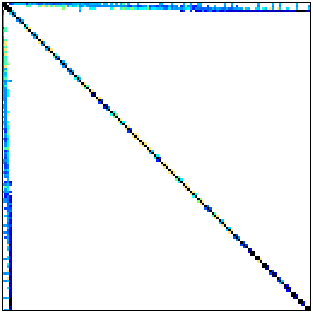
\includegraphics[width=.7\textwidth, keepaspectratio, clip]{Images/ch3/matrices/bundle1.png}
		\subcaption{bundle1}
		\label{Subfigure:comparing-decomposition-implementations-speedup-comparison-between-CM-and-different-ICMs-matrix-bundle1}
	\end{subfigure}%
	\begin{subfigure}{.5\textwidth}
		\centering
		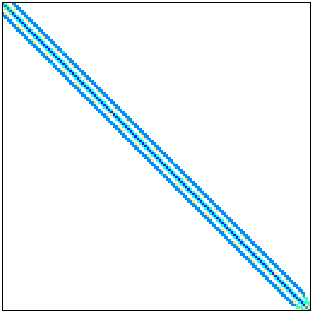
\includegraphics[width=.7\textwidth, keepaspectratio, clip]{Images/ch3/matrices/s1rmq4m1.png}
		\subcaption{s1rmq4m1}
		\label{Subfigure:comparing-decomposition-implementations-speedup-comparison-between-CM-and-different-ICMs-matrix-s1rmq4m1}
	\end{subfigure}
	\caption{Nonzero element pattern of the \textit{bundle1} and \textit{s1rmq4m1} matrices. Taken from \emph{The University of Florida Sparse Matrix Collection} \cite{Davis2011}.}
	\label{Figure:comparing-decomposition-implementations-speedup-comparison-between-CM-and-different-ICMs-matrices-bundle1-s1rmq4m1}
\end{figure}

\par As can be seen from Figure~\ref{Subfigure:comparing-decomposition-implementations-speedup-comparison-between-CM-and-different-ICMs-matrix-s1rmq4m1}, matrix \textit{s1rmq4m1} has nonzero elements on and near its main diagonal. Thus, the matrices arising from the decomposition ($ \mathbb{L} $ and $ \mathbb{U} $, or $ \mathbb{Z} $) will also have elements mainly around their main diagonals. From the perspective of ICM$ x $, this means that the majority of elements requiring computation are found within diagonal sections, therefore, more iterations are required to process them. On the other hand, non-diagonal sections do not require as many iterations as they contain mostly zeros. Consequently, ICM$ x $ can leverage the fact that each diagonal section has the device's resources available to itself and that non-diagonal sections are processed in fewer iterations which results in a fast decomposition of the input matrix. In other words, ICM$ x $ is efficient at decomposing n-diagonal sparse matrices, i.e. matrices that have a small number (n) of nonzero diagonals near the main nonzero diagonal. For the \textit{s1rmq4m1} matrix - using either precision - the optimal number of threads per block is either $ 16 \times 16 $ or $ 32 \times 32 $.
\par Similarly, the main diagonal of the \textit{bundle1} matrix (Figure~\ref{Subfigure:comparing-decomposition-implementations-speedup-comparison-between-CM-and-different-ICMs-matrix-bundle1}) is also densely populated with nonzero elements. However, it also has nonzero elements in its first few rows and columns. Subsequently, the non-diagonal sections that compute these elements require more iterations in order to be processed. Nevertheless, since the matrix's remaining elements are mostly zero, the other non-diagonal sections require a few iterations - if any - to process their elements. Note that the speedup for \textit{bundle1} is greater than the speedup for \textit{s1rmq4m1} due to the large difference in matrix dimensions which causes significant problems for CM.

\begin{wrapfigure}{r}{.5\textwidth}
	\centering
	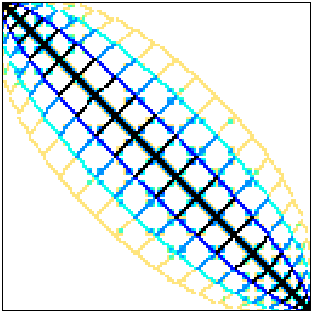
\includegraphics[width=.35\textwidth, keepaspectratio, clip]{Images/ch3/matrices/na5.png}
	\caption{Nonzero element pattern of the \textit{Na5} matrix. Taken from \emph{The University of Florida Sparse Matrix Collection} \cite{Davis2011}.}
	\label{Figure:comparing-decomposition-implementations-speedup-comparison-between-CM-and-different-ICMs-matrix-na5}
\end{wrapfigure}

When it comes to suboptimal performance, the speedup of ICM$ x $ was noticeably low on all dense matrices when using double precision. Since the used dense matrices contain only nonzero elements, every section needed many iterations to be computed which in turn meant that, overall, more iterations were needed to process the entire matrix. For context, the \textit{Cejka5943} dense matrix was decomposed by ICM32 in 44.53 seconds (using double precision), whereas the \textit{Na5} matrix (Figure~\ref{Figure:comparing-decomposition-implementations-speedup-comparison-between-CM-and-different-ICMs-matrix-na5}) was decomposed in 0.12 seconds. \\
The reason behind this stark difference in execution times is that the \textit{Na5} matrix has more so an n-diagonal nonzero element structure with minor protrusions in the center. However, the protrusions do not impact the performance severely since the concentration of nonzero elements on the main diagonal is greater than that of the outer diagonals. Therefore, ICM$ x $ also benefits from the fact that, overall, fewer iterations are required to decompose the entire matrix. \\
When single precision was used, the noticeable difference in speedup between sparse and dense matrices was not as prominent. \\
While the reason behind the significant speedup difference between single and double precision for ICM$ x $ on dense matrices remains unproven, high-speed shared memory access and generally faster operations using single precision are suspected to be the root causes.

\begin{figure}[ht!]
	\centering
	\begin{subfigure}{.5\textwidth}
		\centering
		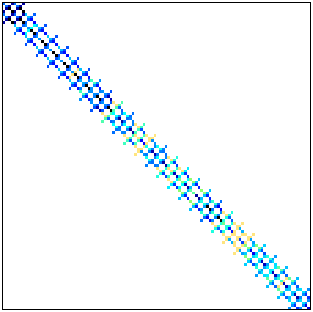
\includegraphics[width=.7\textwidth, keepaspectratio, clip]{Images/ch3/matrices/bcsstk03.png}
		\subcaption{bcsstk03}
		\label{Subfigure:comparing-decomposition-implementations-speedup-comparison-between-CM-and-different-ICMs-of-the-implementations-matrix-bcsstk03}
	\end{subfigure}%
	\begin{subfigure}{.5\textwidth}
		\centering
		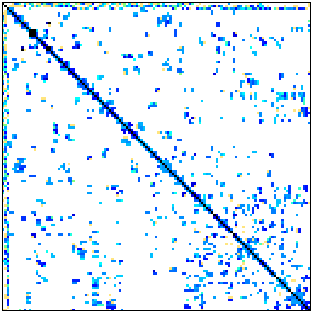
\includegraphics[width=.7\textwidth, keepaspectratio, clip]{images/ch3/matrices/rail_5177.png}
		\subcaption{rail\_5177}
		\label{Subfigure:comparing-decomposition-implementations-speedup-comparison-between-CM-and-different-ICMs-matrix-rail_5177}
	\end{subfigure}
	\caption{Nonzero element pattern of the \textit{bcsstk03} and \textit{rail\_5177} matrices. Taken from \emph{The University of Florida Sparse Matrix Collection} \cite{Davis2011}.}
	\label{Figure:comparing-decomposition-implementations-speedup-comparison-between-CM-and-different-ICMs-matrices-rail_5177-bcsstk03}
\end{figure}

In terms of sparse matrices, ICM$ x $ achieved higher speedups on all with some exceptions, for example, the \textit{bcsstk03} (Figure~\ref{Subfigure:comparing-decomposition-implementations-speedup-comparison-between-CM-and-different-ICMs-matrix-bcsstk03}) and \textit{rail\_5177} (Figure~\ref{Subfigure:comparing-decomposition-implementations-speedup-comparison-between-CM-and-different-ICMs-matrix-rail_5177}) matrices despite the former's nonzero element structure being favorable to ICM$ x $. As Table~\ref{Table:comparing-decomposition-implementations-matrices-used-for-benchmarks-14-selected-matrices} lists, the dimensions of the \textit{bcsstk03} matrix are $ 112\times 112 $ which is advantageous for the sequential implementation of CM, as there are fewer steps to perform. Furthermore, since the matrix was already present in host memory, CM's decomposition procedure began without delay. On the other hand, for ICM$ x $, the matrix first had to be copied to the device memory and, additionally, the pre-kernel overhead subroutine of ICM$ x $ took - in this case - relatively valuable time to complete. This, combined with the fact that the strength of the iterative algorithm lies in the GPU's ability to process larger datasets, indicates that CM is more suitable for decomposing smaller matrices.

\par When it comes to the \textit{rail\_5177} matrix, irrespective of the fact that its main diagonal is heavily populated with nonzero elements, there are other nonzero elements interspersed in a seemingly random fashion throughout the matrix. Therefore, similarly to dense matrices, the non-diagonal sections of this matrix also require more iterations in order to be processed.

\begin{wrapfigure}{r}{.5\textwidth}
	\centering
	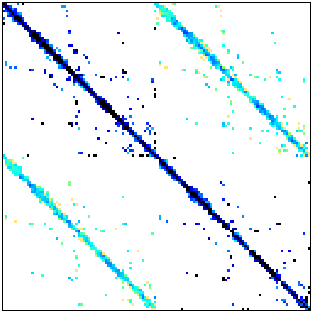
\includegraphics[width=.35\textwidth, keepaspectratio, clip]{images/ch3/matrices/legresley_2508.png}
	\caption{Nonzero element pattern of the \textit{LeGresley\_2508} matrix. Taken from \emph{The University of Florida Sparse Matrix Collection} \cite{Davis2011}.}
	\label{Figure:comparing-decomposition-implementations-speedup-comparison-between-CM-and-different-ICMs-matrix-legresley_2508}
\end{wrapfigure}

Additionally, when comparing the speedup between single and double precision for ICM16 and ICM32 relative to ICM8, unexpected behavior can be seen for the \textit{LeGresley\_2508} matrix (Figure~\ref{Figure:comparing-decomposition-implementations-speedup-comparison-between-CM-and-different-ICMs-matrix-legresley_2508}). When double precision is used, the speedup of ICM16 and ICM32 decreased drastically compared to single precision and compared to the decrease in performance of ICM8. Since $ 1/10 $ of the matrix dimensions are 250.8, \code{sectionSize} is set to \code{256} - the edge of the interval. Thus, \code{sectionSize} is the same for ICM8, ICM16, and ICM32 as their respective \code{BLOCK\_SIZE} is a divisor of \code{256}. Therefore, from the perspective of software, the only difference between the implementations in this instance - except for the precision - is the different \code{BLOCK\_SIZE}. It can be argued that ICM8 performed better due to the greater granularity of its thread blocks combined with the smaller size of the matrix. The greater granularity stems from the fact that ICM8 had 32 blocks assigned to each SM, whereas ICM16 had 8 and ICM32 had  2 - the A100 has a maximum of 2048 threads (64 warps; 32 blocks) per SM \cite{soj8qSRbfefUdi8Y}. This means that if the GPU would run out of resources in terms of concurrently active threads, then ICM8 would fair better as its smaller blocks could fill up the remaining resources more tightly (detailed in \textit{\nameref{Paragraph:theory-CUDA-thread-management-grid}} in Section~\ref{Paragraph:theory-CUDA-thread-management-grid}).

\par This effect is only observed when decomposing smaller matrices that have a nonzero element structure similar to that of \textit{LeGresley\_2508}, i.e. matrices with nonzero elements on the main diagonal and nonzero elements interspersed elsewhere.

\par Figure~\ref{Graph:comparing-decomposition-implementations-performance-of-implementations-across-all-matrices-speedup-single-double-precision} seems to further confirm this suspicion for certain matrices where ICM8 outperforms ICM16 and ICM32 when double precision is used. For matrices with larger dimensions, this effect would be mitigated since being able to utilize a few additional blocks would not amount to such a drastic difference in performance. Furthermore, the non-coalesced global memory access present for ICM8 (more so than for ICM16) becomes apparent when decomposing larger matrices - especially when using single precision.

\paragraph{ICM8} In general, ICM8 was faster than CM, however, when its speedup is compared to that of ICM16 and ICM32, there is a difference in performance. In terms of single precision, the speedups achieved seem to be slightly lower for the first 10 matrices (\textit{bcsstk03} to \textit{Cejka5943}), however, they are considerably lower the larger the matrix dimensions become. Specifically, for matrices that require fewer iterations in order to be decomposed, for example, \textit{s1rmq4m1}, \textit{Na5}, and \textit{bundle1}. \\
Since the execution time for these matrices when using single precision was - at worst - 0.5 seconds for each (0.9 for double precision), loading elements from global to shared memory became a bottleneck. The reason behind this stems from the fact that threads in blocks are divided into warps by their \code{threadIdx.x} index. Thus, when reading from shared memory, threads in a warp should - ideally - access neighboring global memory addresses. Since elements of the \code{DenseMatrix} instance are stored in row-major order on the GPU, each warp in ICM8 loads elements from global memory in the following way: the first 8 threads of the warp read data from neighboring addresses, the next 8 threads of the warp read from other neighboring addresses, in other words, they are not found near the first 8 addresses (unless the matrix dimensions are $ 8\times 8 $) - this is non-coalesced access to memory. In this instance, the non-coalesced access is similar to the example depicted in the upper image of Figure~\ref{Sub-figure:theory-CUDA-global-memory-non-coalesced-access-2}. Therefore, as mentioned in the figure's caption, instead of the threads in a warp performing one transaction to global memory, they will perform $ 32/8 = 4 $ sequential transactions (detailed in \textit{\nameref{Paragraph:theory-CUDA-memory-management-global-memory}} in Section~\ref{Paragraph:theory-CUDA-memory-management-global-memory}). \\
This means that non-coalesced access to global memory occurs for ICM8 and ICM16, however, the latter will only perform $ 32/16 = 2 $ sequential transactions. On the other hand, this defect is not present for ICM32 as the threads of a warp access \code{BLOCK\_SIZE = 32} neighboring addresses in global memory. Apart from this behavior being noticeable in Figure~\ref{Graph:comparing-decomposition-implementations-speedup-comparison-between-CM-and-different-ICMs-single-precision}, it is also apparent for double precision when the vertical axis is not $ \log $-scaled, as shown in Figure~\ref{Graph:comparing-decomposition-implementations-speedup-comparison-between-CM-and-different-ICMs-double-precision-non-ylog} (ICM32 performed better than ICM16 which outperformed ICM8).

\begin{figure}[ht!]
	\centering
	\tikzset{mark options={mark size=2.0, line width=0.5pt},font=\small}
	\begin{tikzpicture}
		\begin{axis}
			[
			,width=0.85\textwidth
			,height=0.45\textwidth
			,axis x line*=bottom
			,axis y line*=left
			,xlabel=\textbf{Matrix}
			,x label style={at={(axis description cs:0.575,-0.35)}}
			,ylabel=\textbf{Speedup}
			,xmin=-.5, xmax=13.5
			,ymax=2100
			,xtick=data
			,ytick={1, 500, 1000, 1500, 2000}
			,xticklabels={bcsstk03,494\_bus,LeGresley\_2508,Cejka2842,rail\_5177,c-31,s3rmt3m3,s1rmq4m1,Na5,Cejka5943,fp,Cejka7580,bundle1,Cejka10793}
			,x tick label style={rotate=45,anchor=east,yshift=-6pt,align=right}
			,ymajorgrids
			,legend pos=outer north east
			]
			\addplot[black,mark=triangle*] table [x=id, y=cm-speedup, col sep=comma] {resources/plot-csv-files/14-matrices-double-precision-rci.csv};
			\addplot[red,mark=x] table [x=id, y=icm8-speedup, col sep=comma] {resources/plot-csv-files/14-matrices-double-precision-rci.csv};
			\addplot[green!60!black,mark=square*] table [x=id, y=icm16-speedup, col sep=comma] {resources/plot-csv-files/14-matrices-double-precision-rci.csv};
			\addplot[blue,mark=triangle*] table [x=id, y=icm32-speedup, col sep=comma] {resources/plot-csv-files/14-matrices-double-precision-rci.csv};
			\legend{CM, ICM8, ICM16, ICM32}
		\end{axis}
	\end{tikzpicture}
	\caption{Speedup comparison between the decomposition times of CM and the ICM$ x $ implementations on the set of matrices (Table~\ref{Table:comparing-decomposition-implementations-matrices-used-for-benchmarks-14-selected-matrices}) using \textbf{double} precision.}
	\label{Graph:comparing-decomposition-implementations-speedup-comparison-between-CM-and-different-ICMs-double-precision-non-ylog}
\end{figure}

\paragraph{CM}\label{Paragraph:comparing-decomposition-implementations-speedup-comparison-between-CM-and-different-ICMs-CM-speedup-description}
In Figure~\ref{Graph:comparing-decomposition-implementations-speedup-comparison-between-CM-and-different-ICMs-single-double-precision} it can be seen that CM took more time to decompose most of the benchmarked matrices. However, an interesting result arises when comparing CM and ICM8 for double precision. Specifically, for 3 out of the 14 matrices, ICM8 was slower than CM as it achieved the following speedups: 0.09 for \textit{bcsstk03}, 0.92 for \textit{Cejka7580}, and 0.96 for \textit{Cejka10793}. While the result for \textit{bcsstk03} is not surprising given the matrix's dimensions, the others are. The most likely reason for the lower performance is the non-coalesced access to global memory which is most prominent for ICM8. \\
Nevertheless, since the algorithm used for CM is sequential and computes every element of the resulting decomposed matrix $ \mathbb{Z} $ regardless of its value, then there is no difference in how it computes matrices with distinct nonzero element structures. Thus, it can be concluded that the performance of CM is determined more so by the dimensions of a matrix, rather than its nonzero element structure.
\par Overall, the decomposition of matrices using single precision was faster compared to double precision. However, the difference in speed is not clearly visible in either Figure~\ref{Graph:comparing-decomposition-implementations-speedup-comparison-between-CM-and-different-ICMs-single-double-precision} (due to the vertical axis being $ \log $-scaled) or Figure~\ref{Graph:comparing-decomposition-implementations-speedup-comparison-between-CM-and-different-ICMs-double-precision-non-ylog} (due to the range of the speedup factor being too great for the values to be distinguishable). For this reason, the raw execution times for single and double precision are included in Table~\ref{Table:comparing-decomposition-implementations-speedup-comparison-between-CM-and-different-ICMs-execution-times-single-precision} and Table~\ref{Table:comparing-decomposition-implementations-speedup-comparison-between-CM-and-different-ICMs-execution-times-double-precision} respectively.

\begin{table}[ht!]
	\centering
	\begin{tabular}{|>{\footnotesize}l|>{\raggedleft\arraybackslash\footnotesize}r|>{\raggedleft\arraybackslash\footnotesize}r|>{\raggedleft\arraybackslash\footnotesize}r|>{\raggedleft\arraybackslash\footnotesize}r|}
		\hline
		\multicolumn{1}{|>{\centering\footnotesize}c|}{Matrix} & \multicolumn{1}{>{\centering\footnotesize}c|}{CM} & \multicolumn{1}{>{\centering\footnotesize}c|}{ICM8} & \multicolumn{1}{>{\centering\footnotesize}c|}{ICM16} & \multicolumn{1}{>{\centering\footnotesize}c|}{ICM32} \\ \hline
		bcsstk03        & \cellcolor{green!25}0.0002 &  0.0022 &                     0.0020 &                     0.0022 \\
		494\_bus 		&                     0.0292 &  0.0049 &                     0.0053 & \cellcolor{green!25}0.0043 \\
		LeGresley\_2508 &                     4.2193 &  0.0793 & \cellcolor{green!25}0.0498 &                     0.0531 \\
		Cejka2842		&                     6.2210 &  3.0391 & \cellcolor{green!25}2.1182 &                     2.1412 \\
		rail\_5177      &                    55.1124 &  1.4350 & \cellcolor{green!25}1.0669 &                     1.1022 \\
		c-31		    &                    59.3208 &  0.1598 &                     0.1330 & \cellcolor{green!25}0.1327 \\
		s3rmt3m3        &                    61.9867 &  0.1450 & \cellcolor{green!25}0.1133 &                     0.1684 \\
		s1rmq4m1        &                    67.8509 &  0.0641 & \cellcolor{green!25}0.0502 &                     0.0505 \\
		Na5             &                    62.3995 &  0.0817 & \cellcolor{green!25}0.0636 &                     0.0649 \\
		Cejka5943		&                    90.1114 &  0.7035 &                     0.5230 & \cellcolor{green!25}0.4856 \\
		fp              &                   179.7054 &  0.5278 &                     0.3980 & \cellcolor{green!25}0.3690 \\
		Cejka7580		&                   151.7981 & 12.2164 &                     3.0289 & \cellcolor{green!25}2.2853 \\
		bundle1         &                   617.5120 &  0.4853 &                     0.3425 & \cellcolor{green!25}0.3041 \\
		Cejka10793      &                   643.3462 &  9.2837 &                     2.8510 & \cellcolor{green!25}2.2107 \\ \hline
	\end{tabular}
	\caption{The execution time (in seconds) of decomposition for all implementations on the set of matrices (Table~\ref{Table:comparing-decomposition-implementations-matrices-used-for-benchmarks-14-selected-matrices}) using \textbf{single} precision. The fastest time for each matrix is highlighted in green.}
	\label{Table:comparing-decomposition-implementations-speedup-comparison-between-CM-and-different-ICMs-execution-times-single-precision}
\end{table}

\begin{table}[ht!]
	\centering
	\begin{tabular}{|>{\footnotesize}l|>{\raggedleft\arraybackslash\footnotesize}r|>{\raggedleft\arraybackslash\footnotesize}r|>{\raggedleft\arraybackslash\footnotesize}r|>{\raggedleft\arraybackslash\footnotesize}r|}
		\hline
		\multicolumn{1}{|>{\centering\footnotesize}c|}{Matrix} & \multicolumn{1}{>{\centering\footnotesize}c|}{CM} & \multicolumn{1}{>{\centering\footnotesize}c|}{ICM8} & \multicolumn{1}{>{\centering\footnotesize}c|}{ICM16} & \multicolumn{1}{>{\centering\footnotesize}c|}{ICM32} \\ \hline
		bcsstk03        & \cellcolor{green!25}0.0003 &                     0.0027 &                     0.0026 &                       0.0027 \\
		494\_bus 		&                     0.0299 &                     0.0084 & \cellcolor{green!25}0.0070 &                       0.0082 \\
		LeGresley\_2508 &                     4.3542 & \cellcolor{green!25}0.2055 &                     0.4805 &                       0.6118 \\
		Cejka2842		&                     6.9110 &                     4.5995 &                     3.6436 & \cellcolor{green!25}  3.4559 \\
		rail\_5177      &                    67.9030 &                     3.0109 &                     2.3882 & \cellcolor{green!25}  2.1754 \\
		c-31		    &                    72.3863 &                     0.4913 &                     0.4166 & \cellcolor{green!25}  0.3349 \\
		s3rmt3m3        &                    74.0106 &                     0.3704 &                     0.2997 & \cellcolor{green!25}  0.2577 \\
		s1rmq4m1        &                    81.2749 &                     0.1059 &                     0.0843 & \cellcolor{green!25}  0.0714 \\
		Na5             &                    67.2166 &                     0.1543 &                     0.1365 & \cellcolor{green!25}  0.1243 \\
		Cejka5943		&                   104.6150 &                    70.8865 &                    56.2768 & \cellcolor{green!25} 44.5275 \\
		fp              &                   154.8232 &                     0.9641 &                     0.7715 & \cellcolor{green!25}  0.6287 \\
		Cejka7580		&                   159.6421 &                   172.9549 &                   138.9242 & \cellcolor{green!25}107.8041 \\
		bundle1         &                   679.3846 &                     0.8859 &                     0.6648 & \cellcolor{green!25}  0.5079 \\
		Cejka10793      &                   699.9634 &                   731.9412 &                   556.0243 & \cellcolor{green!25}419.1401 \\ \hline
	\end{tabular}
	\caption{The execution time (in seconds) of decomposition for all implementations on the set of matrices (Table~\ref{Table:comparing-decomposition-implementations-matrices-used-for-benchmarks-14-selected-matrices}) using \textbf{double} precision. The fastest time for each matrix is highlighted in green.}
	\label{Table:comparing-decomposition-implementations-speedup-comparison-between-CM-and-different-ICMs-execution-times-double-precision}
\end{table}

From the results presented in Table~\ref{Table:comparing-decomposition-implementations-speedup-comparison-between-CM-and-different-ICMs-execution-times-single-precision}, it can be concluded that ICM32 is the most suitable implementation for decomposing matrices using single precision. In terms of double precision, the same statement could be made when looking at Table~\ref{Table:comparing-decomposition-implementations-speedup-comparison-between-CM-and-different-ICMs-execution-times-double-precision}. However, since the results presented in the mentioned tables were only a small subset of all results, verification of this claim is required for the entire set of 63 matrices.

\subsection{Performance of Implementations Across All Matrices}\label{Subsection:comparing-decomposition-implementations-performance-of-implementations-across-all-matrices}
This section shows the speedup comparison and accuracy of results using both single and double precision for the decomposition implementations listed in Section~\ref{Section:comparing-decomposition-implementations-benchmarked-implementations} across the entire set of 63 matrices. The benchmarks were run on the platform specified in Table~\ref{Table:comparing-decomposition-implementations-benchmark-platform-specifications}. To illustrate how ICM$ x $ compares to CM on matrices that increase in size, the matrices in the graphs were sorted from smallest to largest. The speedup comparison between CM and ICM$ x $ can be found in Figure~\ref{Graph:comparing-decomposition-implementations-performance-of-implementations-across-all-matrices-speedup-single-double-precision} and the accuracy of the results can be found in Figure~\ref{Graph:comparing-decomposition-implementations-performance-of-implementations-across-all-matrices-accuracy-single-double-precision}. All graphs in this section have a $ \log $-scaled vertical axis as the range of values was too great to present any coherent data.

\paragraph{Speedup} As shown in Figure~\ref{Graph:comparing-decomposition-implementations-performance-of-implementations-across-all-matrices-speedup-single-double-precision}, in terms of speedup compared to CM, the ICM$ x $ implementations achieved similar results.

\begin{figure}[ht!]
	\centering
	\tikzset{mark options={mark size=1.5},font=\small}
	\begin{subfigure}{\textwidth}
		\begin{tikzpicture}
			\begin{axis}
				[
				,width=\textwidth
				,height=0.45\textwidth
				,axis x line*=bottom
				,axis y line*=left
				,xlabel=\textbf{Matrix ID}
				,ylabel=\textbf{Speedup} ($ \log $ scale)
				,x label style={at={(axis description cs:0.46,-.1)}}
				,xmin=-1, xmax=63
				,ymode=log
				,ymajorgrids
				,legend style={at={(0.5,1.15)},anchor=north,cells={anchor=east},legend columns=-1}
				]
				\addplot[black,mark=*] table [x=id, y=cm-speedup, col sep=comma] {resources/plot-csv-files/63-matrices-single-precision-rci.csv};
				\addplot[red,mark=*] table [x=id, y=icm8-speedup, col sep=comma] {resources/plot-csv-files/63-matrices-single-precision-rci.csv};
				\addplot[green!60!black,mark=*] table [x=id, y=icm16-speedup, col sep=comma] {resources/plot-csv-files/63-matrices-single-precision-rci.csv};
				\addplot[blue,mark=*] table [x=id, y=icm32-speedup, col sep=comma] {resources/plot-csv-files/63-matrices-single-precision-rci.csv};
				\legend{CM, ICM8, ICM16, ICM32}
			\end{axis}
		\end{tikzpicture}
		\subcaption{Single precision}
		\label{Graph:comparing-decomposition-implementations-performance-of-implementations-across-all-matrices-speedup-single-precision}
	\end{subfigure}
	\vspace{0.25cm}
	\begin{subfigure}{\textwidth}
		\begin{tikzpicture}
			\begin{axis}
				[
				,width=\textwidth
				,height=0.45\textwidth
				,axis x line*=bottom
				,axis y line*=left
				,xlabel=\textbf{Matrix ID}
				,ylabel=\textbf{Speedup} ($ \log $ scale)
				,x label style={at={(axis description cs:0.46,-.1)}}
				,xmin=-1, xmax=63
				,ymode=log
				,ymajorgrids
				,legend style={at={(0.5,1.15)},anchor=north,cells={anchor=east},legend columns=-1}
				]
				\addplot[black,mark=*] table [x=id, y=cm-speedup, col sep=comma] {resources/plot-csv-files/63-matrices-double-precision-rci.csv};
				\addplot[red,mark=*] table [x=id, y=icm8-speedup, col sep=comma] {resources/plot-csv-files/63-matrices-double-precision-rci.csv};
				\addplot[green!60!black,mark=*] table [x=id, y=icm16-speedup, col sep=comma] {resources/plot-csv-files/63-matrices-double-precision-rci.csv};
				\addplot[blue,mark=*] table [x=id, y=icm32-speedup, col sep=comma] {resources/plot-csv-files/63-matrices-double-precision-rci.csv};
				\legend{CM, ICM8, ICM16, ICM32}
			\end{axis}
		\end{tikzpicture}
		\subcaption{Double precision}
		\label{Graph:comparing-decomposition-implementations-performance-of-implementations-across-all-matrices-speedup-double-precision}
	\end{subfigure}
	\caption{Speedup comparison between CM and ICM$ x $ implementations on the entire set of 63 matrices using both single and double precision. Matrix ID signifies the ID of the matrices after they have been sorted according to their dimension from smallest to largest. The vertical axis is $ \log $-scaled for better visibility of differences between implementations.}
	\label{Graph:comparing-decomposition-implementations-performance-of-implementations-across-all-matrices-speedup-single-double-precision}
\end{figure}

Specifically, when single precision was used, all ICM$ x $ implementations were faster in 54/63 cases. In terms of double precision, ICM32 and ICM16 were faster in 53/63, and ICM8 was faster in 51/63 cases. In other words, contrary to the results of decomposition performance on the subset of 14 matrices presented in Section~\ref{Subsection:comparing-decomposition-implementations-speedup-comparison-between-CM-and-different-ICMs}, these results show that CM outperformed ICM$ x $ in more cases than just one. Although, it must be mentioned that the matrices on which CM performed better than ICM$ x $ did have dimensions between $ 27\times 27 $ and $ 415\times 415 $ (with the two exceptions for ICM8 detailed in \textit{\nameref{Paragraph:comparing-decomposition-implementations-speedup-comparison-between-CM-and-different-ICMs-CM-speedup-description}} in Section~\ref{Paragraph:comparing-decomposition-implementations-speedup-comparison-between-CM-and-different-ICMs-CM-speedup-description}).

\par When it comes to single precision, disregarding the fact that all ICM$ x $ implementations were faster in the same number of cases, a lack of performance of ICM8 can be seen. It appears that the issue with non-coalesced access to global memory made a difference. This is further supported by the fact that after a certain point (matrix 46) ICM8 appears to be consistently falling behind ICM32 - especially noticeable for the larger dense matrices when using single precision (the three dips in speedup after matrix 55 in Figure~\ref{Graph:comparing-decomposition-implementations-performance-of-implementations-across-all-matrices-speedup-single-precision}).

\par In terms of double precision, the performance of ICM$ x $ appears more consistent. The general rule of ICM8 performing worse than ICM16 and ICM32 for larger matrices still stands and the performance of ICM16 for matrices past matrix 30 is - in the majority of cases - less than that of ICM32. The dips in the speedup of ICM$ x $ for matrices past matrix 25 are caused by the dense matrices found in the set.

Additionally, Table~\ref{Table:comparing-decomposition-implementations-performance-of-implementations-across-all-matrices-total-execution-time-single-double-precision} shows the total time required by each implementation to decompose the set of 63 matrices using both single and double precision. The data in this table provides further support to the claim made at the end of Section~\ref{Subsection:comparing-decomposition-implementations-speedup-comparison-between-CM-and-different-ICMs} which stated that ICM32 is the most suitable implementation for single and double precision.

\begin{table}[ht!]
	\centering
	\renewcommand{\arraystretch}{1.5}
	\begin{tabular}{|>{\footnotesize}l|>{\raggedleft\arraybackslash\footnotesize}r|>{\raggedleft\arraybackslash\footnotesize}r|>{\raggedleft\arraybackslash\footnotesize}r|>{\raggedleft\arraybackslash\footnotesize}r|}
		\hline
		\multicolumn{1}{|>{\centering\footnotesize}c|}{Precision} & \multicolumn{1}{>{\centering\footnotesize}c|}{CM} & \multicolumn{1}{>{\centering\footnotesize}c|}{ICM8} & \multicolumn{1}{>{\centering\footnotesize}c|}{ICM16} & \multicolumn{1}{>{\centering\footnotesize}c|}{ICM32} \\ \hline
		Single        & 2,393.09 &    35.88 &  17.36 & \cellcolor{green!25} 13.84 \\
		Double 		  & 2,635.45 & 1,000.27 & 772.29 & \cellcolor{green!25}592.19 \\ \hline
	\end{tabular}
	\caption{The total execution time (in seconds) taken by each implementation to decompose the set of 63 matrices (Table~\ref{Table:comparing-decomposition-implementations-matrices-used-for-benchmarks-14-selected-matrices}) on the RCI compute cluster specified in Table~\ref{Table:comparing-decomposition-implementations-benchmark-platform-specifications} using single and double precision. The fastest time for each precision is highlighted in green.}
	\label{Table:comparing-decomposition-implementations-performance-of-implementations-across-all-matrices-total-execution-time-single-double-precision}
\end{table}

\paragraph{Accuracy of results} While this part is the other key factor of the implementation (the first being speed of execution), it serves more as a means to verify that the presented performance does not come at the cost of drastically inaccurate results. Figure~\ref{Graph:comparing-decomposition-implementations-performance-of-implementations-across-all-matrices-accuracy-single-double-precision} shows the maximum difference between the input matrix $ \mathbb{A} $ and the multiplication of the decomposed matrices produced by the implementations ($ \mathbb{L} $ and $ \mathbb{U} $, or $ \mathbb{Z} $), i.e.

\begin{equation}
	\max\left| \mathbb{A} - \mathbb{L}\mathbb{U}\right| \nonumber \,.
\end{equation}

In other words, the matrix that results from multiplying the matrices obtained from the decomposition ($ \mathbb{L} $ and $ \mathbb{U} $) should - ideally - be the same as the input matrix ($ \mathbb{A} $). The values presented in this part are the largest differences between the actual results and the ideal results.
\par For this project, the maximum difference will also be referred to as the \textit{error}. Similarly to the previous figures, the vertical axis is $ \log $-scaled to present the results more clearly. The graphs in the figures only show data for ICM$ x $ as the accuracy of the results did not differ for the ICM$ x $ implementations.

\begin{figure}[ht!]
	\centering
	\tikzset{mark options={mark size=1.5},font=\small}
	\begin{subfigure}{\textwidth}
		\begin{tikzpicture}
			\begin{axis}
				[
				,width=0.98\textwidth % Slightly slimmer than \textwidth to avoid warning in console for overfull \hbox
				,height=0.45\textwidth
				,axis x line*=bottom
				,axis y line*=left
				,xlabel=\textbf{Matrix ID}
				,ylabel=\textbf{Max. difference} ($ \log $ scale)
				,x label style={at={(axis description cs:0.46,-.1)}}
				,xmin=-1, xmax=63
				,ymode=log
				,ymajorgrids
				,legend style={at={(0.5,1.15)},anchor=north,cells={anchor=east},legend columns=-1}
				]
				\addplot[black,mark=*] table [x=id, y=cm-Adiff, col sep=comma] {resources/plot-csv-files/63-matrices-single-precision-rci.csv};
				\addplot[red,mark=*] table [x=id, y=icmx-Adiff, col sep=comma] {resources/plot-csv-files/63-matrices-single-precision-rci.csv};
				\legend{CM, ICM$ x $}
			\end{axis}
		\end{tikzpicture}
		\subcaption{Single precision}
		\label{Graph:comparing-decomposition-implementations-performance-of-implementations-across-all-matrices-accuracy-single-precision}
	\end{subfigure}
	\vspace{0.25cm}
	\begin{subfigure}{\textwidth}
		\begin{tikzpicture}
			\begin{axis}
				[
				,width=0.98\textwidth % Slightly slimmer than \textwidth to avoid warning in console for overfull \hbox
				,height=0.45\textwidth
				,axis x line*=bottom
				,axis y line*=left
				,xlabel=\textbf{Matrix ID}
				,ylabel=\textbf{Max. difference} ($ \log $ scale)
				,x label style={at={(axis description cs:0.46,-.1)}}
				,xmin=-1, xmax=63
				,ymode=log
				,ymajorgrids
				,legend style={at={(0.5,1.15)},anchor=north,cells={anchor=east},legend columns=-1}
				]
				\addplot[black,mark=*] table [x=id, y=cm-Adiff, col sep=comma] {resources/plot-csv-files/63-matrices-double-precision-rci.csv};
				\addplot[red,mark=*] table [x=id, y=icmx-Adiff, col sep=comma] {resources/plot-csv-files/63-matrices-double-precision-rci.csv};
				\legend{CM, ICM$ x $}
			\end{axis}
		\end{tikzpicture}
		\subcaption{Double precision}
		\label{Graph:comparing-decomposition-implementations-performance-of-implementations-across-all-matrices-accuracy-double-precision}
	\end{subfigure}
	\caption{The accuracy of results achieved by CM and ICM$ x $ implementations on the entire set of 63 matrices using both single and double precision. In this instance, the term "accuracy" refers to the maximum difference of $ \left| \mathbb{A} - \mathbb{L}\mathbb{U} \right| $ where $ \mathbb{A} $ is the input matrix and $ \mathbb{L} $ and $ \mathbb{U} $ are the matrices obtained from the decomposition procedure. The higher the maximum difference, the lower the accuracy of the results (the higher the error). Matrix ID signifies the ID of the matrices after they have been sorted according to their dimension from smallest to largest. The vertical axis is $ \log $-scaled for better visibility of differences between implementations. Note that the vertical axes of both graphs do not cover the same range.}
	\label{Graph:comparing-decomposition-implementations-performance-of-implementations-across-all-matrices-accuracy-single-double-precision}
\end{figure}

Overall, it seems that the accuracy of results produced by both approaches (CM and ICM$ x $) is similar, nevertheless, values for both single and double precision will be analyzed.
\subparagraph{Single precision} The statistical analysis of the accuracy of results for single precision is presented using a collection of basic statistical indexes in Table~\ref{Table:comparing-decomposition-implementations-performance-of-implementations-across-all-matrices-accuracy-statistical-indexes-single-precision}.

\begin{table}[ht!]
	\centering
	\renewcommand{\arraystretch}{1.5}
	\begin{tabular}{|>{\footnotesize}l|>{\raggedleft\arraybackslash\footnotesize}r|>{\raggedleft\arraybackslash\footnotesize}r|}
		\hline
		\multicolumn{1}{|>{\centering\footnotesize}c|}{Accuracy index} & \multicolumn{1}{>{\centering\footnotesize}c|}{CM} & \multicolumn{1}{>{\centering\footnotesize}c|}{ICM$ x $} \\
		\hline
		Average   &   4,540,350.594 &    36,830.430 \\
		Maximum   & 268,435,500.000 & 2,097,152.000 \\
		Minimum   &           0.000 &         0.000 \\
		Median    &           0.125 &         0.031 \\
		Std. dev. &  33,580,198.190 &   262,296.394 \\
		\hline
	\end{tabular}
	\caption{Statistical indexes for the accuracy of the results obtained from the decomposition procedure performed by CM and ICM$ x $ using single precision. The accuracy of the results was rounded to three decimal places as that was sufficient to portray the characteristics of the dataset.}
	\label{Table:comparing-decomposition-implementations-performance-of-implementations-across-all-matrices-accuracy-statistical-indexes-single-precision}
\end{table}

The values from the table present the problem of using single precision. Even though CM is a sequential algorithm and should provide the exact solution the results produced by it can be drastically different from those expected. Specifically, the average error for CM was 4,540,350.594 which is not usable. On the other hand, since the median is 0.125, and the smallest difference is 0 it seems that the large average was caused by a few extreme values. This claim is further supported by the maximum error achieved by CM which is 268,435,500.
\par For ICM$ x $, the average error was 36,830.43 which is significantly lower than that of CM. Furthermore, the maximum error and median value of errors achieved by ICM$ x $ are all lower than that of CM. Additionally, the standard deviation is 128 times smaller than that of CM.
\par In summary, all of the facts mentioned for the accuracy of results when using single precision can be used to further promote the claim made at the end of \textit{\nameref{Subsection:theory-LU-decomposition-numerical-method}} in Section~\ref{Subsection:theory-LU-decomposition-numerical-method}: "\textit{Since Crout's method is direct, it can be theorized that rounding errors may result in it providing less accurate results compared to its numerical modification}". In other words, for single precision, the results suggest that ICM$ x $ is more accurate than CM. However, since the set contained only 63 matrices, further benchmarks on larger sets are required to verify this claim.

\subparagraph{Double precision} Similarly to single precision, the statistical analysis of the accuracy of results for double precision is presented using a collection of basic statistical indexes in Table~\ref{Table:comparing-decomposition-implementations-performance-of-implementations-across-all-matrices-accuracy-statistical-indexes-double-precision}.

\begin{table}[ht!]
	\centering
	\renewcommand{\arraystretch}{1.5}
	\begin{tabular}{|>{\footnotesize}l|>{\raggedleft\arraybackslash\footnotesize}r|>{\raggedleft\arraybackslash\footnotesize}r|}
		\hline
		\multicolumn{1}{|>{\centering\footnotesize}c|}{Accuracy index} & \multicolumn{1}{>{\centering\footnotesize}c|}{CM} & \multicolumn{1}{>{\centering\footnotesize}c|}{ICM$ x $} \\
		\hline
		Average   & 0.0045                   & 0.0398                   \\
		Maximum   & 0.2500                   & 2.0000                   \\
		Minimum   & 0.0000                   & 0.0000                   \\
		Median    & 2.3283$\times 10^{-10}$  & 4.6566$\times 10^{-10}$ \\
		Std. dev. & 0.0314                   & 0.2566                   \\
		\hline
	\end{tabular}
	\caption{Statistical indexes for the accuracy of the results obtained from the decomposition procedure performed by CM and ICM$ x $ using double precision. The accuracy of the results was rounded to four decimal places to portray the characteristics of the dataset. Furthermore, some values were simply too small and as such, they were listed using scientific notation.}
	\label{Table:comparing-decomposition-implementations-performance-of-implementations-across-all-matrices-accuracy-statistical-indexes-double-precision}
\end{table}

Unlike the accuracy of results for single precision, the results achieved using double precision were less erroneous. The average error in the results produced by CM was 0.0045, the maximum error was 0.25 and the minimum error was 0. Furthermore, the median error was at a very accurate $2.33\times 10^{-10}$. However, the most drastic difference when comparing the errors of CM between single and double precision is the standard deviation. For the former, the deviation of errors was 33,580,198.19, whereas for the latter it was 0.0314.
\par When comparing CM to ICM$ x $ for double precision, it can be seen that the roles have switched and that ICM$ x $ is now the less-accurate implementation across all indexes. For ICM$ x $, the average error is 8 times larger than that of CM and its median is double that of CM. Furthermore, the standard deviation of errors for ICM$ x $ is also 8 times greater than that of CM.
\par Ultimately, it can be concluded that CM is the format that produces more accurate matrices when using double precision. However, the performance of CM remains to be multitudes lower than that of ICM$ x $. Further benchmarks on real-life problems are required to determine whether the errors achieved by ICM$ x $ are too severe, or if the speedup compared to CM is worth the slightly more inaccurate results.


\subsection{Comparison of Optimizations}
This section aims to show the evolution of the ICM$ x $ implementations throughout the development process. Since the benchmarks for each optimization were executed during the development process, they were run on a different platform than the results presented in Sections~\ref{Subsection:comparing-decomposition-implementations-speedup-comparison-between-CM-and-different-ICMs} and \ref{Subsection:comparing-decomposition-implementations-performance-of-implementations-across-all-matrices}. The platform used during development was the GP7 compute server (specifications listed in Table~\ref{Table:comparing-decomposition-implementations-comparison-of-optimizations}) which is located in the Faculty of Nuclear Sciences and Physical Engineering of the Czech Technical University in Prague.

\begin{table}[ht!]
	\centering
	\begin{tabular}{|l|l|}
		\hline
		CPU              & Intel(R) Core(TM) i9-9900KF @ 3.60GHz (8 cores, 16 threads) \\
		RAM              & 62GB RAM \\
		GPU              & $ 2\times $ Nvidia GeForce RTX 3060 12GB GDDR6 (360 GByte/s mem. bandwidth) \\
		Operating System & Arch Linux (Kernel Version: 5.18.8) \\
		Compiler         & GCC 12.1.1 \\
		CUDA             & CUDA 11.7 \\ \hline
	\end{tabular}
	\caption{Specifications of GP7 compute server that the benchmarks were run on during development.}
	\label{Table:comparing-decomposition-implementations-comparison-of-optimizations}
\end{table}

Furthermore, a subset of the set of 63 matrices was used for measuring the performance of implementations during development. The reasons for this were the following:

\begin{itemize}
	\item The initial implementations on the GPU were egregiously slow, thus, only sparse matrices smaller than $ 6,000\times 6,000 $ were used at the time.
	\item The final set of 63 matrices underwent numerous changes as newly-found matrices were added throughout the development process. Only once the GPU implementation became adequately performant, larger and dense matrices were added. Once the set was completed, there was an attempt to redo the benchmark results for key optimizations, however, the compute cluster time limit was not sufficient as the decomposition of some dense matrices would require up to two days with the initial GPU implementations.
\end{itemize}

The set of matrices that was used to measure performance during development comprised 50 sparse matrices with dimensions ranging from $ 27\times 27 $ to $ 5,832\times 5,832 $.
\par Other than the key optimizations mentioned in Section~\ref{Section:implementation-optimization}, two additional  will be SMopt to show the effect that the value of \code{sectionSize} can have on both the speed of the computation and the accuracy of the results. Specifically, the key optimizations that will be presented are the following:

\begin{itemize}
	\item \textbf{Base} - The naive implementation (mentioned in \textit{\nameref{Paragraph:implementation-optimization-initial-naive-implementation}} in Section~\ref{Paragraph:implementation-optimization-initial-naive-implementation}).
	\item \textbf{SM} - The first version of the implementation that used shared memory (mentioned in \textit{\nameref{Paragraph:implementation-optimization-calculation-by-tiles-using-shared-memory}} in Section~\ref{Paragraph:implementation-optimization-calculation-by-tiles-using-shared-memory}).
	\item \textbf{SMopt} - The optimized version of the shared-memory implementation (mentioned in \textit{\nameref{Paragraph:implementation-optimization-elimination-of-conditions}} in Section~\ref{Paragraph:implementation-optimization-elimination-of-conditions}).
	\item \textbf{ProcRow5} - The initial implementation of \textit{Processing by row sections} where each section consisted of 512 rows with $ tol = 0.005 $.
	\item \textbf{ProcRow0} - The upgraded version of \textit{Processing by row sections} where $ tol = 0 $.
	\item \textbf{ParSecGPU} - The version of \textit{Processing by parallel sections} where \code{sectionSize} was limited by the capabilities of the GPU (mentioned in \textit{\nameref{Subparagraph:implementation-optimization-section-size-dependent-on-maximum-active-threads}} in Section~\ref{Subparagraph:implementation-optimization-section-size-dependent-on-maximum-active-threads}).
	\item \textbf{ICM32} - The final version of the implementation (mentioned in \textit{\nameref{Paragraph:implementation-decomposition-project-lu-decomposition-iterative-crout-method}} in Section~\ref{Paragraph:implementation-decomposition-project-lu-decomposition-iterative-crout-method}).
\end{itemize}

Note that the tolerance value $ tol $ was set to 0.001 for the \textit{Base} optimization and 0.005 for the \textit{SM}, and \textit{SMopt}.

\paragraph{Execution times} The results will be presented only for double precision and for \code{BLOCK\_SIZE} set to 32. The reason behind this is that the results are shown in order to detail the evolution of the implementation, rather than compare differences in thread-per-block configurations. The execution times for the decomposition of the set of 50 matrices for the optimizations listed above are shown in Figure~\ref{Graph:comparing-decomposition-implementations-comparison-of-optimizations-execution-times-50-matrices-double-precision} (the vertical axis is $ \log $-scaled for clarity) and the total time taken for each optimization to decompose the set of 50 matrices is shown in Table~\ref{Table:comparing-decomposition-implementations-comparison-of-optimizations-total-execution-time}.

\begin{figure}[ht!]
	\centering
	\tikzset{mark options={mark size=1.5},font=\small}
	\begin{tikzpicture}
		\begin{axis}
			[
			,width=0.98\textwidth % Slightly slimmer than \textwidth to avoid warning in console for overfull \hbox
			,height=0.65\textwidth
			,axis x line*=bottom
			,axis y line*=left
			,xlabel=\textbf{Matrix ID}
			,ylabel=\textbf{Execution time [s]} ($ \log $ scale)
			,x label style={at={(axis description cs:0.46,-.1)}}
			,xmin=-1, xmax=50
			,ymode=log
			,ymajorgrids
			,legend style={at={(0.5,1.15)},anchor=north,cells={anchor=east},legend columns=-1}
			]
			\addplot[orange] table [x=id, y=base, col sep=comma] {resources/plot-csv-files/optimizations-50-matrices-double-precision-gp7.csv};
			\addplot[green] table [x=id, y=sm, col sep=comma] {resources/plot-csv-files/optimizations-50-matrices-double-precision-gp7.csv};
			\addplot[blue] table [x=id, y=sm-opt, col sep=comma] {resources/plot-csv-files/optimizations-50-matrices-double-precision-gp7.csv};
			\addplot[black] table [x=id, y=processing-row-005-tol, col sep=comma] {resources/plot-csv-files/optimizations-50-matrices-double-precision-gp7.csv};
			\addplot[gray] table [x=id, y=processing-row-0-tol, col sep=comma] {resources/plot-csv-files/optimizations-50-matrices-double-precision-gp7.csv};
			\addplot[cyan] table [x=id, y=parallel-section-size-gpucap, col sep=comma] {resources/plot-csv-files/optimizations-50-matrices-double-precision-gp7.csv};
			\addplot[red,mark=*] table [x=id, y=icm32, col sep=comma] {resources/plot-csv-files/optimizations-50-matrices-double-precision-gp7.csv};
			\legend{Base, SM, SMopt, ProcRow5, ProcRow0, ParSecGPU, ICM32}
		\end{axis}
	\end{tikzpicture}
	\caption{The execution times (in seconds) taken by each decomposition optimization listed above to decompose the set of 50 matrices using double precision and with \code{BLOCK\_SIZE} set to 32. Matrix ID signifies the ID of the matrices after they have been sorted according to their dimension from smallest to largest. The vertical axis is $ \log $-scaled for better visibility of differences between optimizations.}
	\label{Graph:comparing-decomposition-implementations-comparison-of-optimizations-execution-times-50-matrices-double-precision}
\end{figure}

As can be seen from Figure~\ref{Graph:comparing-decomposition-implementations-comparison-of-optimizations-execution-times-50-matrices-double-precision} the \textit{Base} optimization (orange line) is found above the other optimizations for the majority of matrices, which indicates that it took the most time to decompose each matrix. This fact is further supported by the total time taken by \textit{Base} to decompose the entire set of 50 matrices, which is shown in Table~\ref{Table:comparing-decomposition-implementations-comparison-of-optimizations-total-execution-time}. According to the graph, it would seem that the \textit{SM} and \textit{SMopt} optimizations achieved similar times, however, as can be seen in Table~\ref{Table:comparing-decomposition-implementations-comparison-of-optimizations-total-execution-time}, they were almost 3 and 4 times faster, respectively, than \textit{Base}.

\begin{table}[ht!]
	\centering
	\renewcommand{\arraystretch}{1.5}
	\begin{tabular}{ |c|c|c|c|c|c|c|c| } 
		\hline
		Optimization & Base    & SM     & SMopt & ProcRow5 & ProcRow0 & ParSecGPU & ICM32 \\
		\hline
		Time [s]     & 2,140.83 & 745.15 & 514.91  & 57.79      & 143.68   &  89.91    & 43.88 \\
		\hline
	\end{tabular}
	\caption{The total execution time (in seconds) taken by each optimization to decompose the set of 50 matrices.}
	\label{Table:comparing-decomposition-implementations-comparison-of-optimizations-total-execution-time}
\end{table}

It may be difficult to discern the performance of the remaining optimizations in Figure~\ref{Graph:comparing-decomposition-implementations-comparison-of-optimizations-execution-times-50-matrices-double-precision}. However, the results in Table~\ref{Table:comparing-decomposition-implementations-comparison-of-optimizations-total-execution-time} show that ICM32 was the fastest overall. In general, the table effectively shows how each optimization helped improve the speed of decomposition - specifically the total execution time decreased almost 50 times from \textit{Base} to ICM32. For reference, the total execution time required for ICM32 to decompose this subset of 50 matrices on the RCI compute cluster node (presented in Table~\ref{Table:comparing-decomposition-implementations-benchmark-platform-specifications}) was $ 5.02 $ seconds. \\
It can be seen that the total execution time for \textit{ProcRow5} was $ 57.79 $ seconds, which is significantly faster than the other optimizations (apart from ICM32). The reason behind this is that \textit{ProcRow5} had its tolerance value $ tol $ set to $ 0.005 $, thus, as can be seen in Table~\ref{Table:comparing-decomposition-implementations-comparison-of-optimizations-accuracy-statistical-indexes-double-precision} the accuracy of the results it produced from the set of 50 matrices was not as good as that of ICM32.

\paragraph{Accuracy} In terms of accuracy, Table~\ref{Table:comparing-decomposition-implementations-comparison-of-optimizations-accuracy-statistical-indexes-double-precision} shows that \textit{ProcRow0} achieved the most accurate decomposition results with an average error of 0.0397 and a standard deviation of 0.1752. This is due to the fact that the optimization processed the input matrix by sections comprised of 512 rows. This means that if the tolerance value $ tol $ was set to zero, then the optimization would perform many iterations. However, this gain in accuracy is reflected in the relatively poor performance - shown in Table~\ref{Table:comparing-decomposition-implementations-comparison-of-optimizations-total-execution-time}. Specifically, \textit{ProcRow0} required 143.68 seconds to decompose all 50 matrices.

\begin{table}[ht!]
	\centering
	\renewcommand{\arraystretch}{1.5}
	\begin{tabular}{|>{\footnotesize}l|>{\raggedleft\arraybackslash\footnotesize}r|>{\raggedleft\arraybackslash\footnotesize}r|>{\raggedleft\arraybackslash\footnotesize}r|>{\raggedleft\arraybackslash\footnotesize}r|>{\raggedleft\arraybackslash\footnotesize}r|}
		\hline
		\multicolumn{1}{|>{\centering\footnotesize}c|}{Accuracy index} & \multicolumn{1}{>{\centering\footnotesize}c|}{Base} & \multicolumn{1}{>{\centering\footnotesize}c|}{ProcRow5} & \multicolumn{1}{>{\centering\footnotesize}c|}{ProcRow0} & \multicolumn{1}{>{\centering\footnotesize}c|}{ParSecGPU} & \multicolumn{1}{>{\centering\footnotesize}c|}{ICM32}\\
		\hline
		Average   &  0.8776 & 0.1559                   & 0.0397                   &  0.7004                   & 0.0595                   \\
		Maximum   & 11.0353 & 5.6900                   & 1.0000                   & 29.7813                   & 2.0000                   \\
		Minimum   &  0.0001 & 0.0000                   & 0.0000                   &  0.0000                   & 0.0000                   \\
		Median    &  0.0722 & 8.57963$\times10^{-5} $  & 1.25712$\times10^{-10} $ &  4.07454$\times10^{-10} $ & 1.25712$\times10^{-10} $ \\
		Std. dev. &  1.8660 & 0.8097                   & 0.1752                   &  4.1742                   & 0.2979                   \\
		\hline
	\end{tabular}
	\caption{Statistical indexes for the accuracy of the results obtained from the decomposition procedure performed by the optimizations listed at the beginning of this section. The procedure was done using double precision and with \code{BLOCK\_SIZE} set to 32.}
	\label{Table:comparing-decomposition-implementations-comparison-of-optimizations-accuracy-statistical-indexes-double-precision}
\end{table}

When both speed and accuracy were taken into account, the ICM32 optimization excelled more so in speed, than in accuracy. However, as mentioned before, since the execution time of the most-accurate optimization (\textit{ProcRow0}) was insufficient the procedure used in ICM32 was selected as the optimal choice out of all the optimizations.